% Author: Frank
The protocol is named OverPass as it is aimed to serve as an Overpass Bridge across computationally expensive tasks for Users in a trustworthy manner with lighter Gas cost.
\subsection{Legal Roles} in the OverPass Protocol include Users, Miners, and OverPass instances. An OverPass instance is a Smart Contract instance that follows the OverPass Protocol to provide a platform for Users and Miners to interact regarding a particular Question type, this is referred to as the Kernel Question of an OverPass instance. Users will post computational tasks (of the Kernel Question Type) with a reward through the OverPass instance. Miners will be any Computation Providers that listen to computational tasks posted by Users through the OverPass Contract and cast Advice (unverified solutions) in exchange for incentives. Multiple OverPass contracts of different Kernel Questions can exist on the chain, and any User can post respect question instances to the Contract Instances, while any Miner can listen and cast solutions. 
\subsection{The Trust} in OverPass Protocol is built by assuming the rationality of the Miners: Casting advice cost Gas due to casting itself needs consensus and running of the Verification function of the OverPass Contract but only the optimal answer provider will be rewarded. Computing the correct answer costs little locally and casting a wrong / non-optimal answer won’t cost much less. Therefore rational miners would provide the best possible advice. 
\subsection{The Flow} of the OverPass Protocol is visualized in Figure 1. First, a User calls delegateCompute method with a Question, Reward and Time limit. This Commit will cause the reward to be granted to the first Miner who provided the best Advice within the Time limit. The contact emits an event for any new question posted to inform the Miners who are listing to the Contract address. A miner who is satisfied with the potential reward then casts an answer by calling the Advice method with proof and solution and the Verify method will check the validity and optimality before keeping the new answer as the best answer. 

Once the lifetime of a question has ended, the User can retrieve the best answer so far by calling the getAnswer method with the respective taskId. And the miner can call getIncentive to check if his answer is accepted and obtain a reward if so. 
\begin{figure}[H]
  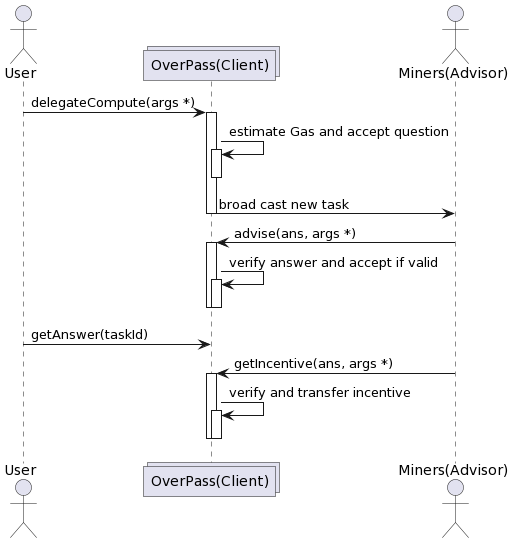
\includegraphics[width=\linewidth]{image/overpass_overview.png}
  \caption{OverPass Protocol Flow}
  \label{fig:boat1}
\end{figure}